\section{Dense Plasma Focus}
\begin{frame} {Plasma Focus Device}
    \begin{figure}
        \centering
        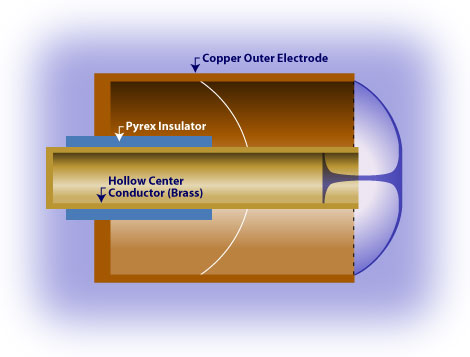
\includegraphics[width=0.7\textwidth]{figures/dfp-device.jpg}
        \caption{Plasma focus device (schematic). Source \cite{plasmauniverse_dense_plasma}}
        \label{fig:dfp-device}
    \end{figure}
\end{frame}

\begin{frame} {How It Works}
    \begin{figure}
        \centering
        \href{https://youtube.com/clip/UgkxWF4zfWfsoU7Gar1u_J0bT1FXJGZnnXn0?si=M5IRMIMCRzouIu3N}{
            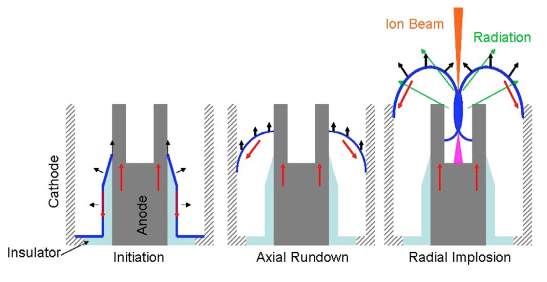
\includegraphics[width=0.7\textwidth]{figures/dfp-phases.png}
        }
        \caption{Three phases of a typical DPF current pulse: initiation via flashover of the insulator, axial run-down phase, and radial implosion of form beams and dense pinch. \cite{krishnan_2012_dense}}
        \label{fig:dfp-phases}
    \end{figure}
\end{frame}

\begin{frame} {X-ray Radiation}
    \begin{itemize}
        \item There are 2 well known mechanisms: line and continuum radiation.
        \item Line radiation: generated by a working gas, or from the interaction between the energetic electrons and impurities.
        \item Continuum radiation: recombination and Bremsstrahlung radiation.
    \end{itemize}
\end{frame}

\begin{frame} {Neutron Emission}
    \begin{itemize}
        \item Two mechanisms: thermal and beam target.
        \item Thermal mechanism: collision of energetic deuterium ions.
        \item Beam target mechanism: interaction of accelerated deuterons with the plasma or background gas.
    \end{itemize}
\end{frame}